% !TEX TS-program = pdflatex
% !TEX encoding = UTF-8 Unicode

% This is a simple template for a LaTeX document using the "article" class.
% See "book", "report", "letter" for other types of document.

\documentclass[12pt]{article} % use larger type; default would be 10pt

\usepackage[utf8]{inputenc} % set input encoding (not needed with XeLaTeX)

%%% Examples of Article customizations
% These packages are optional, depending on whether you want the features they provide.
% See the LaTeX Companion or other references for full information.

%%% PAGE DIMENSIONS
\usepackage{geometry} % to change the page dimensions
\geometry{letterpaper} % or letterpaper (US) or a5paper or....
\geometry{margin=1in} % for example, change the margins to 2 inches all round
% \geometry{landscape} % set up the page for landscape
%   read geometry.pdf for detailed page layout information

\usepackage{graphicx} % support the \includegraphics command and options
\usepackage{wrapfig}
\graphicspath{
{figs/ipe/}
}
% \usepackage[parfill]{parskip} % Activate to begin paragraphs with an empty line rather than an indent

%%% PACKAGES
\usepackage{booktabs} % for much better looking tables
\usepackage{array} % for better arrays (eg matrices) in maths
\usepackage{paralist} % very flexible & customisable lists (eg. enumerate/itemize, etc.)
\usepackage{epstopdf}
\epstopdfsetup{suffix = {}}
\usepackage{siunitx}
\sisetup{unitsep = \cdot}
\usepackage{verbatim} % adds environment for commenting out blocks of text & for better verbatim
\usepackage{subfig} % make it possible to include more than one captioned figure/table in a single float
%\addtokomafont{captionlabel}{\upshape\bfseries} % Bold for caption labels
% These packages are all incorporated in the memoir class to one degree or another...

\usepackage{hyperref}
\usepackage{todonotes}
\usepackage{enumerate}

%%% HEADERS & FOOTERS
\usepackage{fancyhdr} % This should be set AFTER setting up the page geometry
\pagestyle{fancy} % options: empty , plain , fancy
\renewcommand{\headrulewidth}{0pt} % customise the layout...
\lhead{}\chead{}\rhead{}
\lfoot{}\cfoot{\thepage}\rfoot{}

%%% SECTION TITLE APPEARANCE
\usepackage{sectsty}
\allsectionsfont{\sffamily\mdseries\upshape} % (See the fntguide.pdf for font help)
% (This matches ConTeXt defaults)

%%% ToC (table of contents) APPEARANCE
\usepackage[nottoc,notlof,notlot]{tocbibind} % Put the bibliography in the ToC
\usepackage[titles,subfigure]{tocloft} % Alter the style of the Table of Contents
\usepackage{tikz}
\usepackage[framemethod=TikZ]{mdframed}
\renewcommand{\cftsecfont}{\rmfamily\mdseries\upshape}
\renewcommand{\cftsecpagefont}{\rmfamily\mdseries\upshape} % No bold!

%%% END Article customizations

%%% The "real" document content comes below...

\title{BEMOSS: Integrating New IoT Device}
\author{Reece Bachman \and Jordan Ingram \and Robert O'Malley \and \underline{Advisor}: Dr. Suruz Miah
}
%\date{} % Activate to display a given date or no date (if empty),
         % otherwise the current date is printed 

\begin{document}
\maketitle

\section{Project Description}

An internet of things (IoT) network is a network comprised of devices that are often not connected to the internet that have been engineered to have the ability to communicate with each other via wireless network. This allows a single node to control countless physical environments, making the process of running and maintaining a building much simpler. An IOT network will generate a large amount of sensor data that will allow neural networks to be developed for the purpose of smart control of devices. This is the idea behind big data which is a trending topic due to the popularization of internet of things as well as the decrease in the price of memory.
\newline
\newline
The current project is aimed to create a building energy management IoT devices by using Building Energy Management Open Source Software, also known as BEMOSS. We are using BEMOSS as the platform that the devices we make will connect on. Our project is to create the ability for BEMOSS to control a DC motor and to implement a control algorithm to efficiently manage the IOT devices and energy within the network. Having the ability to control a DC motor gives us the opportunity to close curtains, doors, and blinds. Through this, we can further control the climate of a room and building. If a room routinely gets hot around noon, our algorithm would turn on a motor to close the curtains in the room and block the room from the sun. If the building's exterior temperature is below the desired interior temperature, the motor would be used to keep the curtains open as long as possible to increase the usage of the sun's heat. This would add additional cooling and heating to the environment with very low energy consumption. Security could also be improved through this IOT connected device by closing doors during emergencies such as fires and intruder situations. 

The project starts with a very simple attempt to understand BEMOSS and try to get a supported device to work first so that we can understand how to use BEMOSS. Once we have an understanding of how to work with BEMOSS, we shall start doing our own interfacing and working with our own parts.
\newline
\newline
As of September 24, 2018, the BEMOSS does not currently support many electronic devices, such as motors through its IOT In this project, we aim to create an interface device using hardware/software co-design that will be able to fully control a motor from BEMOSS and it is expected to be added to the list of supported devices of the BEMOSS. In doing so, we create a wireless receiver and emitter so that we do not need to connect an expensive single board computer up to the motor just to control it. Once we are able to successfully complete that, XBee will be connected to the single board computer and sends the load commands entered into the system via the control center.

\section{System Architecture}
Figure~\ref{fig:highLevelBemoss} shows the high level system architecture of the current project on customized BEMOSS architecture. As it can be seen from Figure~\ref{fig:highLevelBemoss}  that the proposed BEMOSS architecture consists of five main blocks. The portion at the head of the architecture is the "building energy management center" which is responsible for the command and control of the network based on energy requirements and user demand. The commands are conveyed through a TCP/IP building network. From there, the commands from the TCP/IP network are collected and processed in a wireless sensor central node. This node is responsible for delegating the commands to the array of individual loads in the building through radio frequency communications. The individual loads consist of, but are not limited to, HVAC units, lighting units, fans, and actuators (for example DC motors). These loads are connected to a power grid and operate at the commands received from the central node. 
\newline
\newline
The building energy management control center is run on a computer which is running BEMOSS to communicate with the loads. The wireless sensor central node we are using is an XBee in combination with a single board computer. We are using Raspberry Pi as the single board computer to receive commands from the TCP/IP network and relay the proper load commands to a XBee which communicates with the XBees attached to the loads. 


\begin{figure}
    \centering
    \begin{mdframed}[backgroundcolor=yellow!20,roundcorner=7pt,outerlinecolor= blue!70!black,outerlinewidth=1.2]
    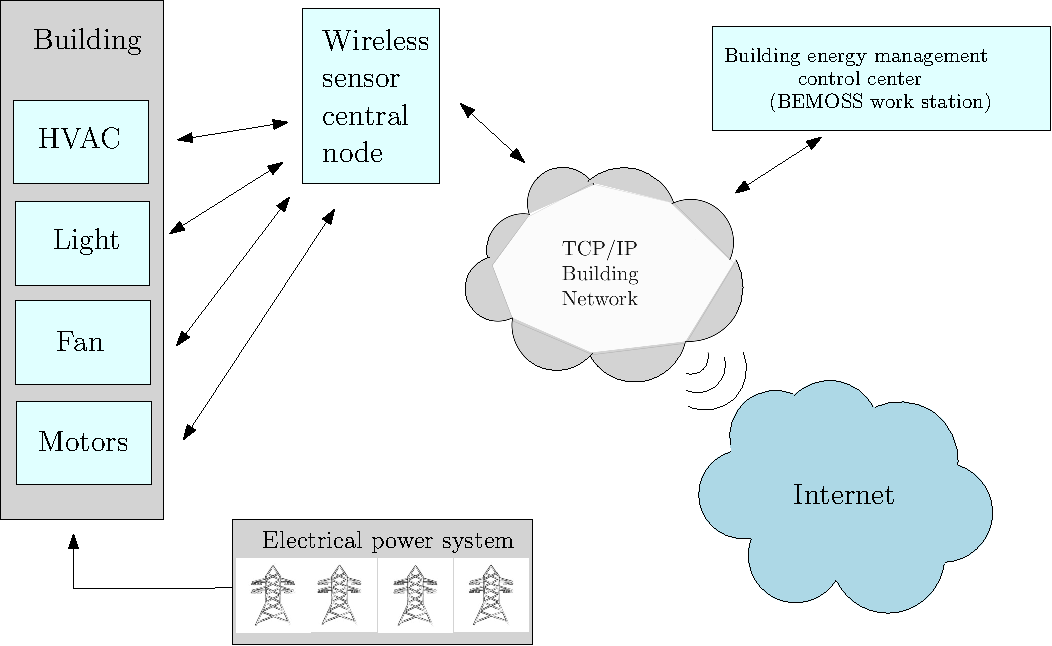
\includegraphics[scale=0.9]{figs/ipe/highLevelBemoss}
    \end{mdframed}
    \caption{High level system architecture of the proposed BEMOSS architecture.}
    \label{fig:highLevelBemoss}
\end{figure}


%\todo[inline]{Describe system level block diagram $\ldots$}
%\missingfigure{System level block diagram.}

\section{Modes of Operations}
\label{sec:modesOfOperations}

The proposed generalized BEMOSS architecture is expected to operate in three different modes: Mode~\#1 (default), Mode~\#2 (user-defined), and Mode~\#3 (energy-efficient usage). A brief description of each of these modes is provided below. %
%
\begin{enumerate}[\textbf{Mode~\#}1]
    \item (Default): This mode will run on non-optimized usage. The plug-and-play devices will be allowed on and off as the user decides to use them. The user will be able to turn their devices on and off through the BEMOSS server.
    \item (User-defined usage): This mode will allow the user to pre-define when they would like the devices to be turned on and off. The user will be able to automate device usage times. 
    \item (Energy-efficient usage): This mode will use a neural network algorithm to automate efficient energy usage.
\end{enumerate}

% \begin{itemize}
%     \item \textbf{DEFAULT} \newline d
%     \item \textbf{USER-DEFINED USAGE} \newline This mode will allow the user to predefine when they would like the devices to be turned on and off. The user will be able to automate device usage times. 
%     \item \textbf{ENERGY EFFICIENT USAGE} \newline This mode will use the neural network algorithm to automate efficient energy usage.
% \end{itemize}


\end{document}

%%% Local Variables:
%%% mode: latex
%%% TeX-master: t
%%% End:
